\documentclass[bachelor]{thesis-uestc}

\title{基于语法树的文档级关系预测算法设计与验证}{Design and Verification of Document-level Relation Extraction Algorithm Based on Syntax Tree}
\author{朱旭东}{Xudong Zhu}
\advisor{康昭\chinesespace 副教授}{Dr. Zhao Kang}
\school{计算机科学与工程学院(网络空间安全学院)}{School of Computer Science and Engineering}
\major{计算机科学与技术}{Computer Science and Technology}
\studentnumber{2020080902004}

\usepackage{graphicx} % for graph
\usepackage{verbatim} % multi-line comment

\begin{document}

\makecover

\begin{chineseabstract}
    文档级关系抽取旨在识别单个文档中实体对之间的关系。
    它需要处理多个句子并对这些句子进行推理。
    最先进的文档级关系抽取使用图形结构来连接文档中的实体,来捕获文档中的实体对的交互。
    但是这些方法没有充分利用在句子级关系抽取中被充分研究的语法信息。
    在本文中我们以将语法树融合到文档级关系抽取中为主要研究内容,重点研究了使用依赖语法树,依存语法树进行文档级关系抽取算法的实现,以及怎么调整依赖语法树和依存语法树的在文档级关系抽取中的权重问题。
    我们利用依存语法树来聚合整个句子信息,并为目标实体对选择有指导意义的句子。
    同时我们利用依赖语法树对整个文档进行细粒度的分析,并选择其中重要的单词增强目标实体对的信息。
    文档级关系抽取将同时利用依赖语法树和依存语法树进行预测。
    通过在不同领域的数据集上的实验结果证明了该方法的有效性。


    \chinesekeyword{文档级关系抽取,依赖语法树,依存语法树,信息抽取}
\end{chineseabstract}

\begin{englishabstract}
    Document-level Relation Extraction (DocRE) aims to identify relation labels between entity pairs within a single document.
    It requires handling several sentences and reasoning over them.
    State-of-the-art DocRE methods use a graph structure to connect entities across the document to capture interaction between entity pairs in the document.
    However, this is insufficient to fully exploit the rich syntax information in the document, which is widely used in sentence-level Relation Extraction(RE).
    In this thesis, we focus on integrating syntax trees into DocRE as the main research topic, and investigate the effective and effient implementation of DocRE algorithms using dependency syntax tree and constituency syntax tree, as well as how to adjust the weight of dependency syntax tree and constituency syntax tree in the extraction.
    It uses constituency syntax to aggregate the whole sentence information and select the instructive sentences for the pairs of targets.
    Meanwhile, it exploits the dependency syntax in a graph structure with constituency syntax enhancement and selects the most important words between entity pairs based on the dependency graph to enhance the information of target entity pairs.
    Finally, DocRE will integrate the dependency syntax and constituency syntax to predict.
    The experimental results on datasets from various domains demonstrate the effectiveness of the proposed method.


    \englishkeyword{Document-level Relation Extraction, Constituency Syntax, Dependency Syntax, Information Extraction}
\end{englishabstract}

\thesistableofcontents

\chapter{绪\hspace{6pt}论}

\section{研究的背景}
\begin{comment}
    课题背景,研究现状, 理论依据,实验基础,发展趋势以及本课题的理论意义
\end{comment}

% 两页

% 关系抽取介绍,包括背景和最近从句子级转移到文档级关系抽取
关系提取是信息提取中的一项关键任务,旨在对非结构化文本中实体对之间的关系模式进行建模。
它有两种特定的场景:句子级关系提取和文档级关系提取。
与句子级关系提取 \cite{sentenceRE-Dixit, sentenceRE-Lyu} 不同,文档级关系提取涉及识别和提取句子边界以外的实体之间的关系,为分析提供了更广泛的上下文,并且更具挑战性。
这项任务可以从非结构化的大型文档(如科学论文、法律合同或新闻文章) \cite{delaunay2023comprehensive} 中自动构建和填充知识库,以更好地理解实体之间的关系。
因此,文档级关系提取更好地满足了实际需求,最近受到了越来越多的关注。\par

% 现在关系抽取的主要方法和存在的一些缺陷

文档级关系抽取的目标是识别在同一文档内的实体对之间的关系。
这是一项复杂的任务,因为它需要理解句子的内容并处理多个句子之间的交互。
由于文档级关系抽取涉及多个句子,现在的研究有三个主要障碍 \cite{9098945}:
\begin{enumerate}
    \item \em{数量更多的潜在关系}: 相比于单个句子,一个文档中包含的实体数量更多。
    由于我们需要预测每两个实体之间的关系,因此潜在的待预测关系随着实体的增加呈指数级别增加。
    \item \em{处理实体共指}: 一个实体通常在一个句子中只出现一次,而在一个文档中,它可以以多种形式出现多次。例如,在图3的句子2和句子3中,"He"是"Marcus Miller"的共同指称。
    \item \em{处理长距离关系}: 在文档级关系抽取中,我们通常需要预测跨句子之间的关系,这可能会导致实体对之间距离过长。
    然而,长句中通常包含不相关甚至有噪声的信息。Huang等人\cite{huang-etal-2021-three} 认为,在大多数情况下,最多只需要三个句子作为识别关系的支持证据。此外,这项工作指出,句子之间的重要性差异很大。不包含任何有价值的信息或关系的句子实际上阻碍了文档的理解。这也是我们这篇论文要解决的主要工作。
\end{enumerate}
\begin{figure}[h]
    \centering
    \caption{文档级关系抽取的一个例子。图片上方是文档内容,文档中实体用不同的颜色标注,下方是文档级关系抽取的结果。}
    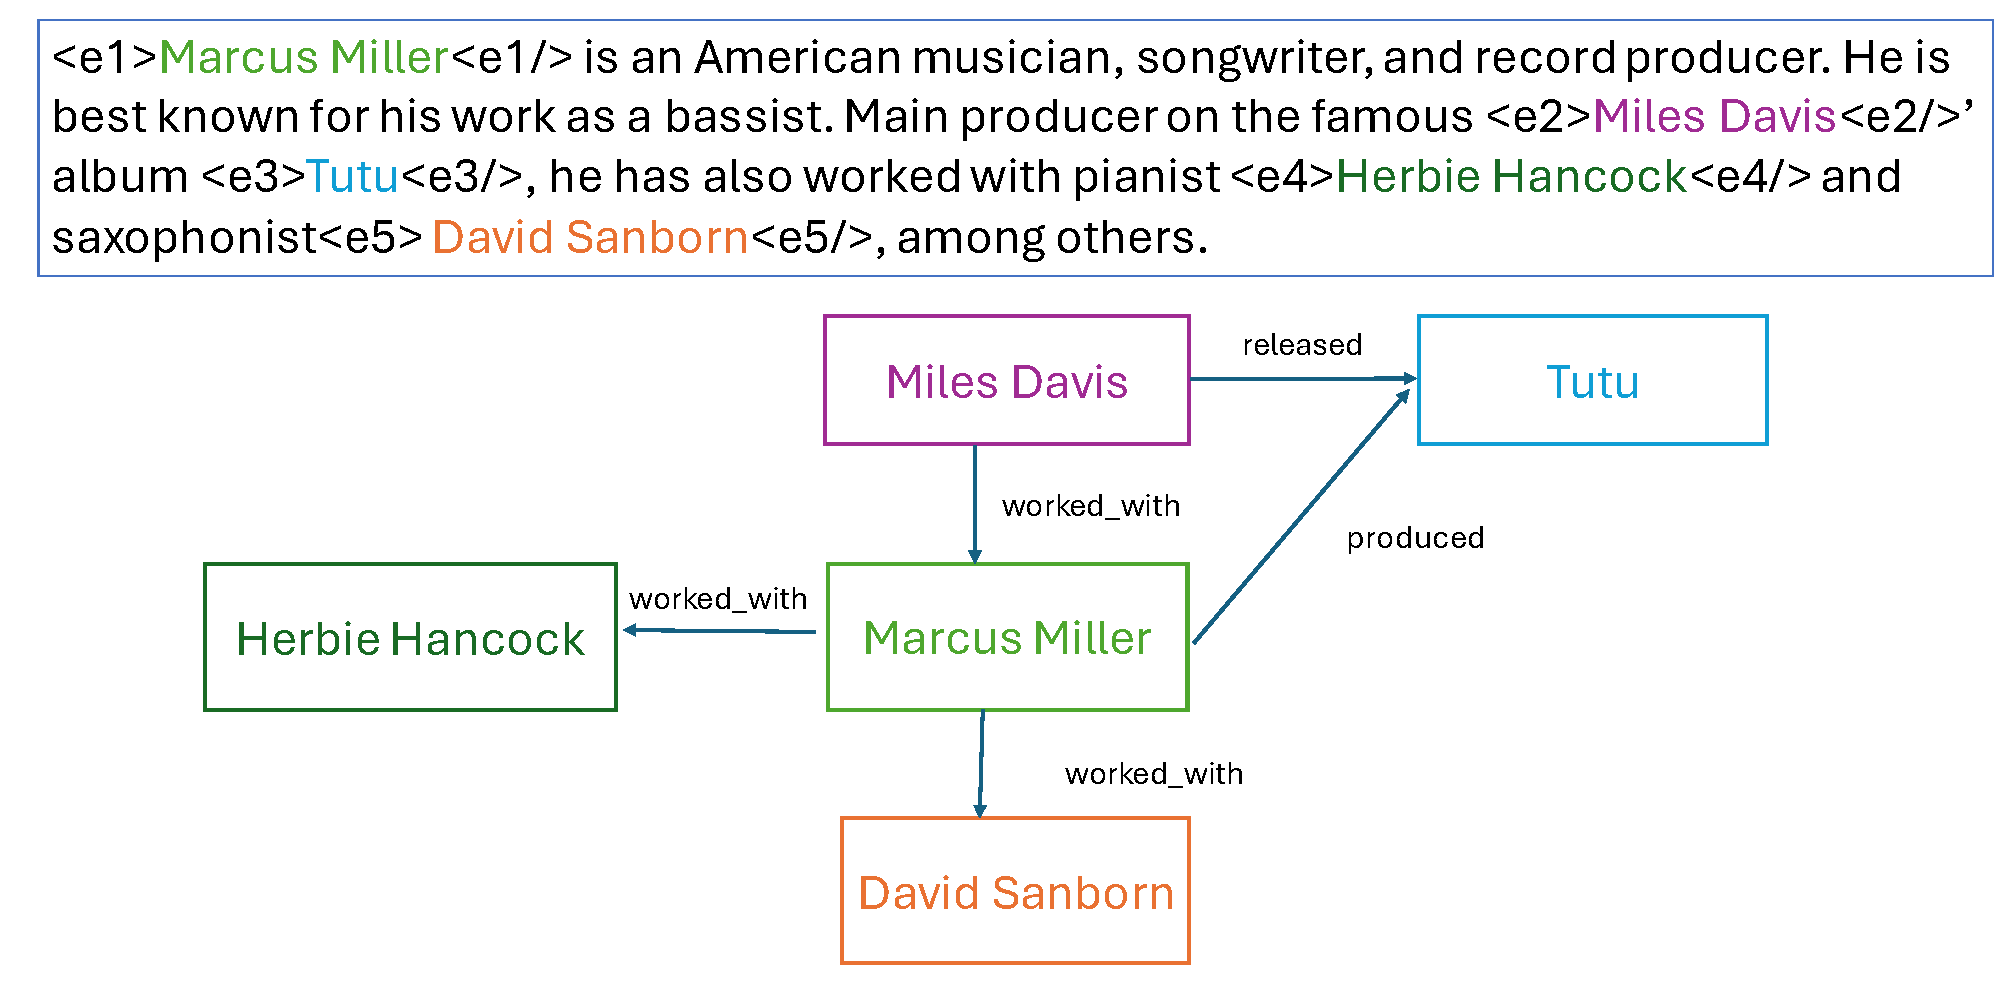
\includegraphics[width=0.8\textwidth]{misc/fig_example.pdf}
\end{figure}\label{fig_example}

图 \ref{fig_example}是一个例子,它包括来自同一文档中的句子级关系和文档级关系。
为了推断"Marcus Miller"和"Herbie Hancock"之间的关系,模型应该能够排除不相关实体的影响,并找出句子3中的"he"一词指的是"Marcus Miller"。
然而,由于现有的文档级关系提取模型 \cite{bai-etal-2021-syntax} 经常会被大量不相关的信息所淹没,从而无法捕捉到类似的关键信息。 \par

由于以上这些原因,本文提出了新的一种文档级关系提取方法,通过融合语法信息作为辅助,来改进文档级关系提取。\par

\section{研究的主要贡献与创新}
% 语法方法是如何帮助文档级关系抽取的,我们的方法大体是怎么做的
本文主要处理文档级关系提取的长距离关系。
由于长句中通常包含无关甚至嘈杂的信息 \cite{gupta2019neural},对于文档级关系提取来说,隐含地学习指导性上下文是不够的 \cite{bai-etal-2021-syntax}。
最近的一些文章通过预训练模型和注意力机制来学习文档中复杂的交互 \cite{huang-etal-2021-three, y2020-coreferential, zhou2021document}, 他们通过创建更复杂、更强大的变体transformer来隐含的捕获实体之间复杂的互动。
但是,更多的方法通过显示捕获实体互动信息来改善文档级关系抽取。他们首先构建由不同节点组成的文档图 (例如实体的提及节点,实体节点,句子节点或者文档节点) \cite{GAIN, liu2023document},将指导性上下文转化为图。
由于语法信息可以通过提供显式语法细化和子内容建模来帮助文档级关系抽取 \cite{duan-etal-2022-just},最近的研究 \cite{sahu2019inter, SagDRE} 采用依赖图来合并语法信息和结构上下文。
他们发现一个精心设计的图形可以帮助模型更好的捕获实体互动信息,缩短实体之间的距离。
然而,正如 \cite{sundararaman2019syntax, bai-etal-2021-syntax}所指出的,尽管预训练模型是用大量真实世界的文本数据进行训练的,但隐式学习的语法与黄金语法之间仍然存在很大差距。
事实上,语法信息在句子级关系抽取中得到了广泛的应用\cite{xu-etal-2016-improved, qin-etal-2021-relation},但在文档级关系抽取场景下尚未得到充分的探索。\par

为了充分利用文档中的语法信息,本文融合了依存语法和依赖语法。
我们主要采用依赖图和依存树来合并额外的语法信息,并使用依存树中的信息来进一步增强依赖图的表示。
依赖语法描述了一个句子中单词之间的依赖关系,这些依赖关系对原始纯文本有很强的补充作用。
而依存语法可以分层合理地组织单个句子的不同单词,消除了枚举不同单词组合的过程,同时保持了分层语法信息。
在树形深度学习模块 \cite{duan-etal-2022-just} 的帮助下,我们可以收集具有适当权重的所有子内容,以解决句间依赖关系并融合依赖语法产生最终关系预测。\par

% 总结,我们的贡献

通过对三个公共文档级关系抽取数据集 (DocRED \cite{DOCRED}、CDR \cite{li2016biocreative} 和GDA \cite{GDA} )的广泛实验下,我们证明我们的算法在很大程度上优于现有方法。
我们在这篇文章中的主要贡献可以总结如下:
\begin{enumerate}
    \item 我们建议利用依存语法树来聚合句子级信息,以弥补依赖语法树中的差距,并通过添加文档节点来改进依赖图,以减少实体对的距离,简化长句交互。
    \item 我们分别用Tree-LSTM和GCN处理转化后的依赖语法和依存语法,并设置一个可学习的参数来调整它们的权重。
    \item 实验结果表明,我们的模型在三个公共文档级关系抽取数据集上的测试优于现有方法,特别是在DocRED上,我们的模型将最先进方法的IgnF1提高了至少1.56\%
\end{enumerate}

\section{研究的结构安排}
本研究的后续方式组织: 第二章主要介绍文档级关系抽取的研究现状,在这一章中,我们对过往的研究结果进行总结。第三章介绍我们的研究工作,包括我们依赖语法和依存语法的使用方式,以及如何调节这两种语法的权重。第四章报告了我们研究的实验结果,包括在三个公共文档级关系抽取数据集上的不同指标的分数,与过往研究的分数对比以及分析;同时包括了对我们方法的每个模块的分析。
\begin{comment}
    课题的方案论证,包括课题的主要任务,功能要求,性能指标等
    课题的工作
    A. 理论课题
(a) 理论基础和原理
(b) 理论分析、推导、数学模型
(c) 模型仿真(含数据、曲线等)

also: 图表的标注先写在图表的上方,明天再次询问这个问题
\end{comment}
\chapter{关系抽取研究}
在这一部分,我们首先对关系抽取进行定义。
然后我们介绍对文档级关系方法的回顾。
\section{关系抽取的定义}
% 一页

在这篇文章中,我们遵循Zhang等人提出的定义 \cite{zhang-etal-2020-document}。
对于每个预测任务,我们有文档$D=\{S_i\}_{i=1}^{n_s}$和实体集合$E=\{e_i\}_{i=1}^{n_e}$。
其中$n_s$是文档中句子的数量,$n_e$是实体的数量,在句子级关系抽取中$n_s$被固定为1,但是在文档级关系抽取中没有限制。
文档中的句子被表示为$S_i=\{w_j\}_{j=1}^{n_w^j}$,其中$w_i$是第$i$个句子中的第$j$个单词。
每一个实体被表示为$E_i=\{m_j\}_{j=1}^{n_w^j}$,其中$m_i$是第$i$个实体中的第$j$个提及。
在句子级别设置中,一个实体只由一个提及表示,即$\forall i \in [1, n_e], e_i = m_i$, 但是在在文档级关系抽取中情况并非如此,其中实体可以通过多次提及来表示。
为了获得实体的固定表示,以前的方法首先对所有提及的嵌入进行平均,即 $e_i = \frac{\sum_{j=1}^{n_m^j} m_j}{n_m^i}$,或者对所有提及的嵌入进行最大池化。
然而,现在的方法都使用更加柔和的logsumexp表示,即 $e_i = \log \sum_{j=1}^{n_m^j} \exp(m_j)$,这样可以促进来自弱提及信息的积累 \cite{jia-etal-2019-document}。
我们也采用这种方式表示每一个实体。\par

文档级关系抽取的目标是正确推断每个实体对$(e_s,e_o)_{s,o = 1, 2, \dots, n_e}; s \neq o$之间的关系。
其中$e_s$是头实体, $e_o$是尾实体。
预测的关系是预定义的关系集合$R$或者$NA$(没有关系)的子集。

\section{文档级关系抽取}
本节介绍了文档级关系抽取的最新进展,重点介绍基于序列的,基于注意力机制的和基于图的文档级关系抽取方法,并分析他们的优缺点。

\subsection{基于序列的文档级关系抽取}
执行文档级关系提取的一种方法是将文档视为一个长的增强的序列,并应用从句子级关系抽取导出的序列模型来识别特定实体之间的关系。

\subsubsection{基于卷积神经网络的文档级关系抽取}
Gu等人 \cite{10.1093/database/bax024}通过两个分离的模型来提取关系。
他们首先将最大熵系统用于句子间的预测,卷积神经网络模型用于句子内的预测。
然后,这两个结果被合并以获得文档级别的关系。
此外,他们还定义了一些启发式规则来从摘要中提取关系,例如将论文标题中提到的所有化学物质(或如有必要,将摘要中最频繁的化学物质)与摘要中提及的所有疾病相关联。\par

李等人 \cite{li2018chemical}
使用递归分段卷积神经网络进行化关系提取,并结合了领域知识、分段策略、注意力机制和多实例学习。
该方法首先利用分段卷积神经网络来捕获单个实例的表示。
然后,使用递归神经网络来聚合实例的表示,从而能够为实体对形成全面的文档级表示。

\subsubsection{结合卷积神经网络和递归神经网络的文档级关系抽取}
Mandya等人 \cite{mandya2018combining}提出了一种长短期记忆和卷积神经网络的组合模型,该模型利用单词嵌入和位置嵌入来提取跨句子的$n$元关系。
长短期记忆模型将结合单词嵌入和位置特征的变换矢量表示作为输入,将输出被馈送到卷积神经网络中。
卷积神经网络被用来提取最重要的特征。
这种方法的优点是独立于复杂的句法特征,如依赖树、共指消解或话语特征。因此被广泛应用到后续的改进模型中。

为了提取基因-疾病相关性,Wu等人 \cite{wu2019renet}还在其方法中结合了门控神经单元。
在这里,卷积神经网络首先使用具有不同宽度的不同滤波器从单词表示中计算句子表示,以捕捉不同的特征。
然后,门控神经单元将它们转换为文档表示。
通过消融实验,他们发现,即使单独的卷积神经网络也可能捕捉到文档的一些重要特征,而额外的门控神经单元层可以提高其性能。
这项研究后来被Su等人 \cite{renet2} 进行了扩展。
在Wu等人的系统之前引入了部分过滤步骤,来删除不包含任何实体对信息和模糊关系的段落。

\subsubsection{以实体为中心的文档级关系抽取}
在传统的句子级关系抽取中,对提及元组进行分类预测就已经足够了,但是在文档级关系抽取中却不是这样。
因为任何实体都可能有多次提及,应用简单的提及级别分类方法会使模型在大量的提及中淹没,导致预测失败。
为了解决这个问题,Jia等人 \cite{jia-etal-2019-document} 提出通过对每个实体元组进行单一关系预测,使用以实体为中心的多尺度预测。它们通过对实体的所有上述表示应用logsumexp来获得实体表示。

\subsubsection{基于序列的文档级关系抽取总结}
这些方法通过将文档视为一个长的增强的序列,将句子级关系抽取的方法自然的映射到文档级关系抽取上。
这些方法的优点是能够处理长文档,并且能够利用跨句子的关系信息。
然而,当待预测实体对涉及到处理长距离并需要多跳推理上下文内容时,这些模型不可避免地会遇到挑战。

\subsection{基于注意力机制的文档级关系抽取}
% 三页

\subsubsection{早期基于注意力机制的文档级关系抽取}
Verga等人\cite{verga-etal-2018-simultaneously} 引入了双仿射关系注意力网络来计算实体之间的关系,它同时预测实体之间的句子内关系和句子间关系。
为了实现这一点,它首先使用transformer层对令牌嵌入进行编码,然后它使用双仿射运算产生实体提及对之间的预测。
最后,它使用logsumexp来汇集每个实体提及级别预测,以获得实体级别预测。
该系统可以针对命名实体识别和关系预测进行联合训练,这可以提高对噪声的鲁棒性; 此外,该系统在编码长序列方面相比于以往的方法更有效。\par

为了缓解正负关系之间的数据不平衡问题,Wang等人\cite{corr} 采用了两步微调过程和预训练模型。前者识别两次提及之间是否存在关系,后者仅使用先前识别的关系事实来训练模型来识别这些实体。\par
为了增强语言表示模型中的共指推理,Ye等人 \cite{y2020-coreferential}在各种下游任务上测试了他们的系统,这其中也包括文档级关系抽取。
他们引入了一种称为提及参考预测的新的预训练任务。
该任务利用了文章中的重复提及,并采用提及参考掩蔽来预测相应的参考,而不是依赖于监督的共同参考数据进行微调。此外,他们引入了基于新的训练目标,以鼓励基于上下文的单词选择和上下文敏感的表示,从而促进共指推理。

\subsubsection{分层注意力模型}
为了将推理信息从实体级聚合到句子级,再聚合到文档级,唐等人 \cite{Tang2020HINHI}使用层次推理网络进行预测。
受Bordes等人 \cite{NIPS2013_1cecc7a7} 中给出的平移约束的启发,该约束对关系三元组$( r, e_s, e_o )$进行了建模。
他们通过将实体提及和关系联合建模,获得了实体级别的表示信息。
然后,他们应用语义匹配方法将实体级推理信息与每个句子向量进行比较,并使用多层双向长短期记忆模型获得句子级信息。
最后,他们重新利用注意力机制来识别关键的句子级推理信息,这有助于以更全面的方式全面表征文档级推理。
虽然这种方法十分有效,但是它的正确性受到广泛质疑,因为在文档级抽取中,两个实体对可以具有多个关系,一个实体可以与多个其他实体具有相同的关系。\par

Kuang等人 \cite{app12031599} 认为,实体对之间的关系通常可以通过几个关键词来推断。
为了从中受益,他们使用自注意记忆模块与预训练模型结合,通过寻找具有高交叉注意力实体对的单词嵌入来捕捉关键词特征。
他们的模型非常简单,在专用和非专用数据集上都取得了很好的改进,并可应用于其他数据集。

\subsubsection{基于实体表示的注意力模型}\label{subsec:entity-based-attention}

Han和Wang \cite{9098945}利用具有类型信息的文档级实体掩码方法来提供更多关于文档级关系预测中实体的信息。
它在预训练模型的嵌入中引入了实体特征,用上下文信息和实体特定信息丰富了实体的表示。
Han和Wang首先使用预训练模型来获得实体提及的上下文化表示。
然后,它使用一次性关系预测方法一次性处理所有实体对,因此文本只编码一次。\par

采用与Jia等人 \cite{jia-etal-2019-document}相同的实体中心主义观点, Yu等人 \cite{yu-etal-2022-relation} 还解释了每一次提及之间的重要性,以代表关于特定关系的实体。
他们使用关系特定提及注意力网络(RSMAN)将每个关系的基本语义合并到关系表示中,然后计算候选关系和给定实体对的提及表示之间的注意力。
通过考虑这些事项,该模型通过对所有提及的表示进行加权聚合来获得实体的合成表示。
这使得模型能够在不同的表示空间中捕获来自多个提及的信息,从而为不同的候选关系产生灵活的、特定于关系的实体表示。
作为一种插入式方法,RSMAN可以用作任何关系预测模型的方法中。\par

如前所述,在文档级关系预测中,一个文档包含多个实体对,这些实体对可以在文档中多次出现,并具有多种可能的关系。
为了解决这些问题,Zhou等人 \cite{Zhao2022DocumentlevelRE}在预训练模型的基础上使用了两种技术:自适应阈值和本地化文本池(ATLOP)。
自适应阈值通过将多标签分类的全局阈值与可学习的依赖于实体的阈值进行切换来为每个实体对确定最佳阈值。
而本地化文本池直接将注意力从预先训练的语言模型转移到有助于确定关系的相关上下文。
这解决了对所有实体对使用相同实体嵌入的问题。
ATLOP通过与当前实体对相关的额外上下文丰富了实体嵌入,实现了更全面的表示,并为DocRE带来了巨大的飞跃。
在我们的方法中,我们也采用了它的这两种技术。\par

\subsubsection{基于远程监督标签的注意力模型}

Xiao等人 \cite{xiao-etal-2020-denoising} 试图通过三个预训练任务来减少远程监督标签中引起的固有噪声:提及实体匹配,关系检测和关系事实对齐。提及实体匹配涉及文档内和文档间的匹配,第一种侧重于在文档内建立共引用连接,而另一种则捕获文档之间的实体关联;关系检测,主要检测被错误标记为负面的正面关系;关系事实对齐确保模型即使以不同的方式表示,仍然为同一实体对生成一致的表示, \par

接着,Tan等人 \cite{tan-etal-2022-document} 提出了一种利用远程监督数据的多步骤方法。首先,他们使用注意力模块作为特征提取器,允许关注逻辑路径中的不同元素,并捕捉关系三元组(关系,头实体和尾实体)之间的相互依赖性。其次,为了处理类的不平衡,他们引入了一种关注长尾类的自适应焦点损失,使它们对整体损失的贡献更大。最后,他们利用知识提炼来弥合手动注释数据和远程监督数据之间的差距。它由一个用少量人工注释数据训练的教师模型组成,该模型对大量远程监督数据生成预测,从而为预训练学生模型提供软标签。

\subsubsection{基于结构推理的注意力模型}

Xu等人 \cite{Xu_Wang_Lyu_Zhu_Mao_2021} 基于当时文档级关系抽取模型的一个问题,即上下文推理和结构推理的阶段是分开的、因此缺乏对上下文表示的结构指导,从而引入了结构化自注意网络(SSAN),将结构依赖性包含在编码网络内和整个系统中。他们利用自注意机制的一个新扩展 \cite{Vaswani2017AttentionIA},通过考虑两个实体结构,一个用于同一句子中的实体对的共现,另一个用于单个实体的共指,有效地对其构建块内和所有网络层自下而上的提及依赖性进行建模。除了实体提及之间的依赖性,Xu等人 \cite{Xu_Wang_Lyu_Zhu_Mao_2021}还使用注意力模块来捕捉实体提及与句内非实体之间的关系。它们包含了一个额外的与注意力模块并行的模块,该模块以上下文化的查询键表示为条件,对结构依赖性进行建模。这种设计使模型能够受益于结构相关性的指导,确保上下文信息和结构信息有效集成。

\subsubsection{基于联合学习的注意力模型}
Ma等人 \cite{ma-etal-2023-dreeam} 解决了学习文档级关系抽取和证据提取的两个问题:高资源消耗和缺乏人工注释数据。他们使用证据引导注意机制进行的文档级关系提取,通过在证据提取上指导ATLOP模型 \cite{zhou2021document}来完成证据提取和节省资源消耗。Ma等人使用手动标注的实体对特定的局部上下文嵌入进行计算,并将注意力权重作为证据得分结合在标记上。这种方法允许他们引入来自证据提取的知识,而不引入额外的可训练参数或昂贵的矩阵计算。为了缓解数据的缺乏,他们使用了与Tan等人 \cite{tan-etal-2022-document} 类似的知识提取技术, 利用远程监督数据来训练学生模型。

\subsubsection{基于注意力的文档级关系抽取模型小结}

综上所述,基于注意力的文档级关系抽取模型的研究已经取得了长足的进步。
目前,除了早期的一些朴素方法,现有的方法大致可以分为以上五类,这些方法可以将实体嵌入、关系嵌入和上下文信息结合起来,以获得比基于序列的模型更好的文档级关系抽取结果。
这些模型的共同特点是使用注意力机制来捕捉不同实体和关系之间的依赖关系,并将它们融合到统一的表示中。
它们的优点在于能够捕捉到实体和关系之间的复杂关系,并能够在不同的表示空间中捕获来自多个提及的信息。
这些模型的缺点是需要它们要么需要额外的远程监督数据,要么需要设计复杂的分层结构。
而且由于实体之间的距离可能较长,它们中大多数方法没有办法有效的处理长距离交互。
然而,它们中的一些思想和假设十分有效(如第\ref{subsec:entity-based-attention} 节的ALTOP的自适应阈值和本地化文本池等),因此在最近的研究中被广泛采用。
\subsection{基于图的文档级关系抽取}
在这一节中,我们首先在第\ref{subsec:early-graph} 节介绍早期的一些图的文档级关系抽取方法。然后我们将现有的基于图的文档级关系抽取模型分为五类:分别在第\ref{subsec:joined-graph}节中介绍了联合任务的图文档级关系抽取方法,在第\ref{subsec:entity-centric-graph}节中介绍了以实体为中心的图文档级关系抽取方法,在第\ref{subsec:heterogeneous-graph}节中介绍了基于异构图的图文档级关系抽取方法,在第\ref{subsec:layered-graph}节中介绍了基于分层网络的图文档级关系抽取方法,在第\ref{subsec:optimal-graph}节中介绍了基于最优图结构的图文档级关系抽取方法。

\subsubsection{早期的图文档级关系抽取方法}\label{subsec:early-graph}
\begin{figure}[htbp]
    \centering
    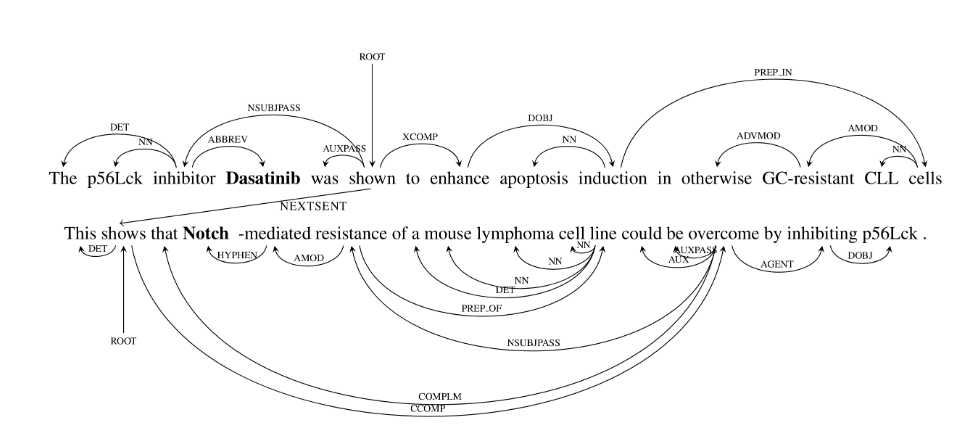
\includegraphics[width=0.8\textwidth]{misc/doc_graph_2017.png}
    \caption{Quirk和Poon \cite{quirk-poon-2017-distant}构建的文档图}
\end{figure}\label{fig:quirk-poon}
Quirk和Poon \cite{quirk-poon-2017-distant} 引入了文档图的概念。它提供了一种统一的方法,通过将单词表示为节点,将一些启发式的关系(例如,依赖关系,邻接关系等)表示为边,来导出对待预测的关系进行分类的特征,图\ref{fig:quirk-poon}是这种文档图的一个示例。
这为文档级关系抽取的所有基于图的方法铺平了道路。
Peng等人 \cite{peng-etal-2017-cross} 决定将这种图表示作为其框架的主干,其中包含一种新的图形长短期记忆模型。
在经典的长短期记忆模型体系结构中,每个单元只有一个前置点(因此只有一个遗忘门)。图形长短期记忆模型的情况并非如此,通过从树形长短期记忆模型 \cite{tai-etal-2015-improved} 中获得灵感,它可以具有多个前置点,包括通过不同边与同一单词连接的点,并为每个单元添加与先例数量一样多的遗忘门。
从输入文本获得的单词嵌入被作为图形长短期记忆模型的输入,该图捕捉每个单词的上下文表示。
然后,实体的上下文表示通过这种图形的连接进行组合,并由关系分类器使用。
在多单词实体的情况下,Peng等人计算其单词表示的平均值来获得实体的嵌入向量,尽管现在大多采用logsumexp操作来获得更好的结果,但这种方法在当时是首创。
至于图形长短期记忆模型的反向传播,他们将文档图拆分为两个有向无环图。
一个有向无环图包含从左到右的线性连接链接相邻的单词以及其他前向指向依赖项(前向传递),而另一个有向无环图则涵盖从右到左的线性连接链接相邻的单词和后向指向依赖性(后向传递) \par

Christopoulou等人 \cite{christopoulou-etal-2018-walk} 提出了一种仅用于句子级关系抽取的基于图的随机行走的神经网络,同时处理多对关系,并将句子表示为向无环图,这种方法的详细过程参见图\ref{fig:christopoulou}。
他们后来在将他们的方法扩展到文档级别,引入部分连接的文档图而不是以前的完全连接的文档,使得文档级关系抽取向前迈出了一大步。
与仅包含实体节点和单个边缘类型的句子级图相比,这种新的文档图由异构类型的节点和边组成,当实体提及可用时,这种方法可以使用多实例学习来进一步提高模型的性能。
节点之间的连接基于预定义的文档级交互,目标是使用图中的其他现有边生成实体到实体的边表示,从而推断实体到实体关系。
在这项任务中,Christopoulou等人 \cite{christopoulou-etal-2019-connecting}还发现,文档级信息有助于找到句内关系。
同年年初,同一团队 \cite{sahu-etal-2019-inter}中提出应用图卷积网络实现消息传递。
在该方法中,利用依赖语法边、相邻句子和单词边、自节点边以及共引用边来构造文档图,以连接句子的依赖树。
Guo等人 \cite{guo-etal-2019-attention}还提出通过注意力引导来扩展关系抽取的图卷积网络结构,以有效地关注任务的相关子图,而不修剪一些重要信息。\par
\begin{figure}
    \centering
    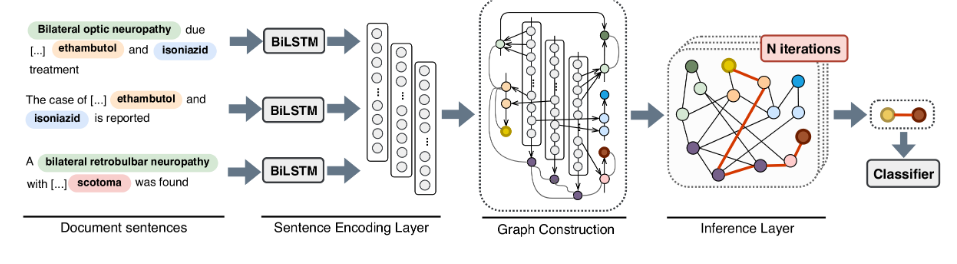
\includegraphics[width=0.8\textwidth]{misc/DAG2018.png}
    \caption{Christopoulou \cite{christopoulou-etal-2018-walk} 等人用于句子级关系抽取的基于图的随机行走的神经网络。该模型对句子进行编码,并将其输入迭代算法,以生成目标实体节点之间的边缘表示。为简洁起见,未显示某些节点连接。}
\end{figure}\label{fig:christopoulou}


根据Quirk和Poon \cite{quirk-poon-2017-distant} 中引入的依赖图,Gupta等人 \cite{Gupta_Rajaram_Schütze_Runkler_2019} 捕捉了两个实体之间的最短依赖路径,同时考虑了句内和句间关系。它们使用双向循环神经网络来表示通过依赖子树的最短依赖路径上的每个单词。
他们提出的方法,基于句子间依赖的神经网络,通过将句子解析树的根节点连接到后续树的根,结合最短依赖路径来处理句子间关系。此外,他们采用了一种增强依赖路径,其中双向循环神经网络对句子间最短依赖路径上每个单词的依赖子树进行建模,然后提取显著的语义特征。
在大多数情况下,增强依赖路径模型比最短依赖路径模型更好,然而,他们没有在DocRE的基准数据集上进行测试。
当将他们的方法与 \cite{peng-etal-2017-cross}进行比较时,他们指出,由于其非循环结构架构,他们的系统更简单、更高效。\par

此外,Minh Tran等人 \cite{minh-tran-etal-2020-dots}发现基于图的过往模型只关注图的边缘表示,而忽略了节点的表示。
因此,这些模型错过了实体及其提及中包含的潜在重要线索,并阻止模型利用节点和边缘表示之间的关系,以及利用实体的表示向量之间的相似性找到相同实体的节点。
因此,他们扩展了Christopoulou等人 \cite{christopoulou-etal-2019-connecting}的EoG模型。
他们通过合并三个损失来提高模型表现:一个用于节点表示,一个用于结点边缘表示一致性,以及一个用于实体提及表示一致性。\par

\subsubsection{基于联合任务的图文档级关系抽取}\label{subsec:joined-graph}

Luan等人的工作 \cite{luan-etal-2019-general}主要集中在联合任务中执行不同的信息抽取任务。
他们首先提出了一个句子级信息抽取系统,使用动态跨度图同时执行命名实体识别,关系抽取和共指消解。
由于模型可以随着新信息添加到输入文本中而更新,因此它能够传播实体共指和关系类型置信度,这有助于跨度表示的迭代细化。
这与以前的模型形成了对比。
在以前的模型中,任务之间的唯一交互发生在共享的第一层长短期记忆模型中。\par

Wang等人 \cite{WANG2021107274}使用一种新颖的修辞结构理论来建立有效的语义联想,以及一套证据推理方法来选择合适的证据,以此来训练他们的话语感知神经关系抽取模型。
通过将关系抽取和证据提取进行联合培训,这种方法缓解对关系抽取的证据缺乏选择和推理能力的问题。\par

在类似的方向上,Xie等人 \cite{xie2022eider}提出通过有效的证据提取和推理阶段融合来增强文档级关系抽取的能力。
在训练步骤中,对模型进行关系抽取和证据提取的联合训练,而在推理过程中,对原始文档和提取证据的预测结果进行组合,这鼓励模型专注于重要句子,同时减少信息损失,强迫模型在句子中进行更多推理,使其能够包含更多关于关系的知识,从而使模型具有更高的性能。
最近的一些工作 \cite{SagDRE, duan-etal-2022-just}, 将文档图和证据提取结合到一起,利用语法信息来辅助进行文档图的构建和证据的提取。但是他们将两者孤立的进行训练,而没有考虑到它们的相互融合。
\par

\subsubsection{以实体为中心的图文档级关系抽取}\label{subsec:entity-centric-graph}

与以实体为中心的注意力模型相似,基于图的文档级关系抽取模型也对实体信息做了扩展。
Zeng等人\cite{GAIN}提出了图聚合和推理网络,该网络结合了由提及级别和实体级图组成的双图设计。
图聚合和推理网络捕捉不同提及之间的复杂互动,并聚合属于同一实体的互动。
这是通过三种类型的边来实现的:一种是执行共指解析的实体内边,一种是对句子中实体之间的交互进行建模的实体间边,以及一种文档边、所有提及节点都连接到文档节点。
通过建立这些关系,文档节点可以有效地处理所有提及,并促进文档和单个提及之间的交互。
它还解决了长距离依赖的挑战,因为文档节点可以作为使用GCN传递消息的枢纽(见图\ref{fig:GAIN})。但是这种方法也有一个显著的缺点,那就是它的计算复杂度过高,无法处理大规模数据集。\par

\begin{figure}
    \centering
    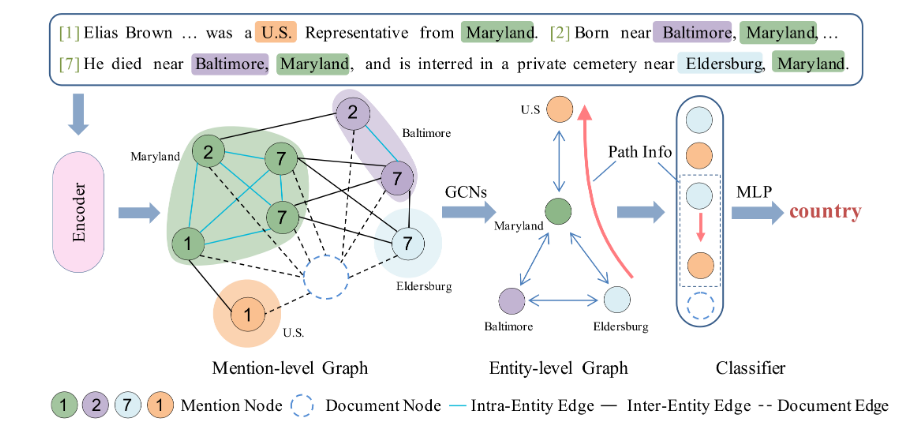
\includegraphics[width=0.8\linewidth]{misc/GAIN.png}
    \caption{图聚合和推理网络的结构 \cite{GAIN}。首先,上下文编码器获得每个单词的上下文化表示。然后,利用提及节点和文档节点构建提及级图。在应用图卷积网络之后,构建了实体级图,其中识别实体之间的路径以进行推理。最后,分类模块利用收集的信息对目标关系进行预测。不同的实体有不同的颜色。}
\end{figure}\label{fig:GAIN}

为了考虑共指信息,Xue等人 \cite{y2020-coreferential}提出了基于图推理网络的文档级关系提取(CorefDRE),通过提及代词聚类直接指示模型学习共指信息。
他们使用提取所有提及代词对,并使用预训练模型计算每个提及代词对的可信度,以减少代词带来的噪声。
CorefDRE首先利用提及代词对及其可信度得分,结合代词节点、提及节点和各种类型的边,构建提及代词可信图。
然后,它将图卷积网络应用于提及代词可信图,以捕获提及和代词的有意义的表示,同时也抑制了可能的噪音,将其转化为同构实体图。
最后,模型聚合图中的节点和边表示,获得用于有效分析和理解的综合表示。\par

与Xue等人 \cite{y2020-coreferential}类似,Li等人 \cite{LI2022109146}介绍了一种基于自监督仿射计算对单词和实体进行聚类的共指图。
这些聚类作为一个节点阵列,能够捕获跨句推理的线索,然后将它们转换为图。
该图将共指图与Zeng等人 \cite{GAIN}提出的提及图相结合,使其成为实体图。
这种模型采用了关系图卷积网络和噪声抑制机制 \cite{y2020-coreferential},产生了同构实体图,这使得即使这种方法允许增强长距离关系的建模,两个图的合并仍然不会引入不希望的噪声。\par

\subsubsection{基于异构图的图文档级关系抽取}\label{subsec:heterogeneous-graph}
基于基于异构图的图文档级关系抽取与基于分层网络的方法有些相似,但是基于异构图的方法更强调使用不同的图形,而不是使用分层网络来辅助文档级关系抽取。
Zhang等人 \cite{zhang-etal-2020-document}提出了第一种双层异构图,有效地将这顺序信息和结构信息结合起来,以促进多跳推理和最终预测。
该模型主要由一个结构建模层组成,考虑了对文档固有结构进行全面编码,包括文档中单词的顺序、语法和层次结构。
关系推理层通过在不同实体之间传播关系信息来促进多跳关系推理。\par

然而,这种模型中的大多数构建了所有实体对之间的关系信息,而不知道它们之间是否存在关系。
因此,Xu等人 \cite{Xu2020DocumentLevelRE}提出使用重构来迫使他们的基于异构的图自注意网络更加关注具有标注关系的实体对的学习。
重构器沿着连接两个实体节点的路径生成一系列节点表示,当实体对之间存在标注关系时,最大化路径的概率。这样可以进一步提高模型的性能。 \par

借鉴前人的工作,Wang等人 \cite{zhang-etal-2020-document} 提出了一种多层异构图神经网络模型。它构造了一个多层异构图,包括单词级图、提及级图和实体级图。前两个图分别使用面向节点类型和边缘类型的异构图注意力网络进行消息传递。
然后,实体级图采用基于门控的路径推理机制来提取多跳关系。
这种方式和我们介绍的基于分层网络的方法就非常相似了。\par

\subsubsection{基于分层网络的图文档级关系抽取}\label{subsec:layered-graph}

为了区分句内推理和句间推理,Kim等人 \cite{app10031181} 在其全局关系提取器中使用了一种分而治之的方法,通过使用两个独立的模型来提取局部和全局关系并构建知识图来完全避免这个问题。
全局关系提取器由一个基于长短期记忆的句子级关系抽取模块和一个负责从局部关系生成知识图的知识图构造器模块组成;两个模型都是交替训练的。\par

Li等人 \cite{li-etal-2021-mrn} 采用基于局部和全局提及的推理网络来区分近距离和远距离实体提及的影响。
他们添加了一个新的共同预测器,利用局部和全局实体表示来联合推理近实体和远距离实体之间的关系。
该模型包括一个二维窗口卷积,用于捕捉关系的实体对之间的局部提及的交互。
此外,模型还添加了一个注意力模块,用于捕捉每对实体提及之间的全局交互,这些实体提及彼此交互以提供局部和全局上下文之间的信息。
该模型获得了很高的性能,证明了句内关系和句间关系之间的相互作用对文档级关系抽取的模型的有效性。\par

在类似的思想下,Zeng等人 \cite{zeng-etal-2021-sire} 强调了文档级关系抽取中处理句内关系和句间关系的常见做法。
由于二者高度相似,这导致在预测这些不同关系类型时缺乏区分性。
而且并非所有的实体对都可以通过路径连接,一些逻辑推理路径可能无法完全捕获在图中,这导致在许多实体对无法被逻辑推理覆盖。
他们的方法将句内推理和句间推理分开。
对于句内关系,他们使用句子级编码器来表示每一个同时出现的实体。通过聚合所有共现实体的关系表示,它们获得了一个最终表示,该表示鼓励句内实体对在其特定上下文中强调局部模式。
为了捕捉句子间的关系,继他们之前的工作 \cite{GAIN}之后,他们采用了文档级编码器和提及级图,使模型能够捕捉全局和局部上下文。
为了选择性地识别可能的跨句关系的句子,他们使用证据选择器,它鼓励句子间实体对选择性地关注为其跨句关系提供支持证据的句子。\par

\subsubsection{基于最优图结构的图文档级关系抽取}\label{subsec:optimal-graph}

Nan等人\cite{nan-etal-2020-reasoning}发现使用共同引用和规则构建图并不总是导致最优的图结构。
因此,他们建议将图结构视为一个潜在变量,并以端到端的方式对其进行归纳,以增强整个文档中的信息聚合。
他们的潜在结构优化模型由一个节点构造函数和一个动态推理器组成,节点构造函数将节点作为每次提及的上下文表示,动态推理器从迭代优化的节点中生成文档级结构。\par

Huang等人 \cite{huang-etal-2021-three}专注于研究在流行数据集中识别关系需要多少句子。
他们发现,在DocRED数据集中,当段落平均由八句话组成时,96.1\%的例子需要不超过三句话作为支持证据,87.7\%的例子甚至只需要两句或更少。
CDR和GDA数据集也进行了类似的计算。
研究人员给出的一种可能的解释是,考虑到人类工作记忆的局限性,关系抽取任务的性质自然局限于有限数量的实体和上下文信息。正如Barreyro等人 \cite{barreyro2012working} 所述,工作记忆在推理任务中尤为重要,但其分离信息块的能力通常限制在四句话左右。
因此,在数据中观察到的三句话信息块的共同模式可能是我们用于相互理解的潜意识策略。
利用这些假设,Huang等人设计了三个启发式规则来从每个文档中提取路径,旨在近似支持证据:连续路径(头和尾实体在三个连续的句子中)、多跳路径(头实体和尾实体分别相隔在长距离的句子中,但可以通过与不同句子中的和头实体和尾实体同时出现的枢轴实体进行连接)和默认路径(所有成对的句子,其中一个包含头实体,另一个包含尾实体)。
即使他们的方法看起来过于简单,但当论文发表时,他们通过将其与双向长短其记忆模型相结合,比一些最先进的方法获得了更好的结果 \cite{nan-etal-2020-reasoning,GAIN},这表明明确选择最佳路径比完全依赖基于图的模型要好。\par

\subsubsection{基于图的文档级关系抽取总结}\label{subsec:graph-neural-network}

基于图的文档级关系抽取方法有着广泛的应用,他们相比于基于注意力的方法有着明显的优势,因为它们可以将关系推理的结构信息结合到图结构中,从而更好地捕捉长距离关系。
然而,这些方法要么使用启发式的图结构,无法捕获原文中的顺序信息\cite{GAIN, Xu2020DocumentLevelRE};要么分别使用依赖性和选区信息捕捉不同粒度的信息来预测不同的任务 \cite{SagDRE, duan-etal-2022-just},但没有将它们结合到一起。
在我们这项研究中,我们通过结合选区和依赖信息,并使用选区树增强依赖图来克服以上缺点。通过引入不同的语法,我们的模型可以融合不同粒度的信息,更好地捕捉长距离关系。

\section{本章小结}

在这一章中,我们深入探讨了围绕文档级关系抽取任务的现有文献的大体方法和他们对应的优缺点。
除了传统的基于序列的方法,我们将基于注意力的方法和基于图的方法各自分为五种。可以观察到,这两类方法有很多相通之处,利于他们都重视实体信息,各自提出一些假设来丰富实体信息。再者二者都重视文档的结构信息,都利用结构信息来辅助推理。
但是,基于图的方法不仅有更优秀的性能,也有着更好的解释性。通过利用语法信息将文档转化为文档图,我们可以更好的捕捉实体对之间的关系,同时缩短实体对之间的距离,简化它们之间交互的同时也能保存足够多的信息。
因此本研究立足于图形的方法来改进文档级关系抽取任务。


\chapter{基于语法树的文档级关系抽取研究}
为了充分利用文档中的语法信息,本文融合了依存语法和依赖语法来改进文档级关系抽取。
我们主要采用依赖图和依存树来合并额外的语法信息,并使用依存树中的信息来进一步增强依赖图的表示。
依赖语法和依存语法描述了语法信息的互补但不同的方面。图 \ref{fig_syn_a}中的依赖图主要用于整合单个句子内的句法信息,该信息与原始纯文本具有很强的互补性,而图\ref{fig_syn_b}中的依存树则分层合理地组织单个句子的不同单词。\par

我们算法的总体架构如图\ref{overview}所示。
我们利用依赖语法和依存语法来构建依赖图和依存树,并利用预训练模型对文档中的单词进行编码。
然后,我们使用树形长短期记忆模型来聚合来自依存树的信息,并通过图神经网络利用依赖图的信息,同时利用依存树来改进依赖图。
我们通过可学习权重来调节依赖图和依存树的关系,以更好的利用这两种语法信息。

\begin{figure*}
    \centering{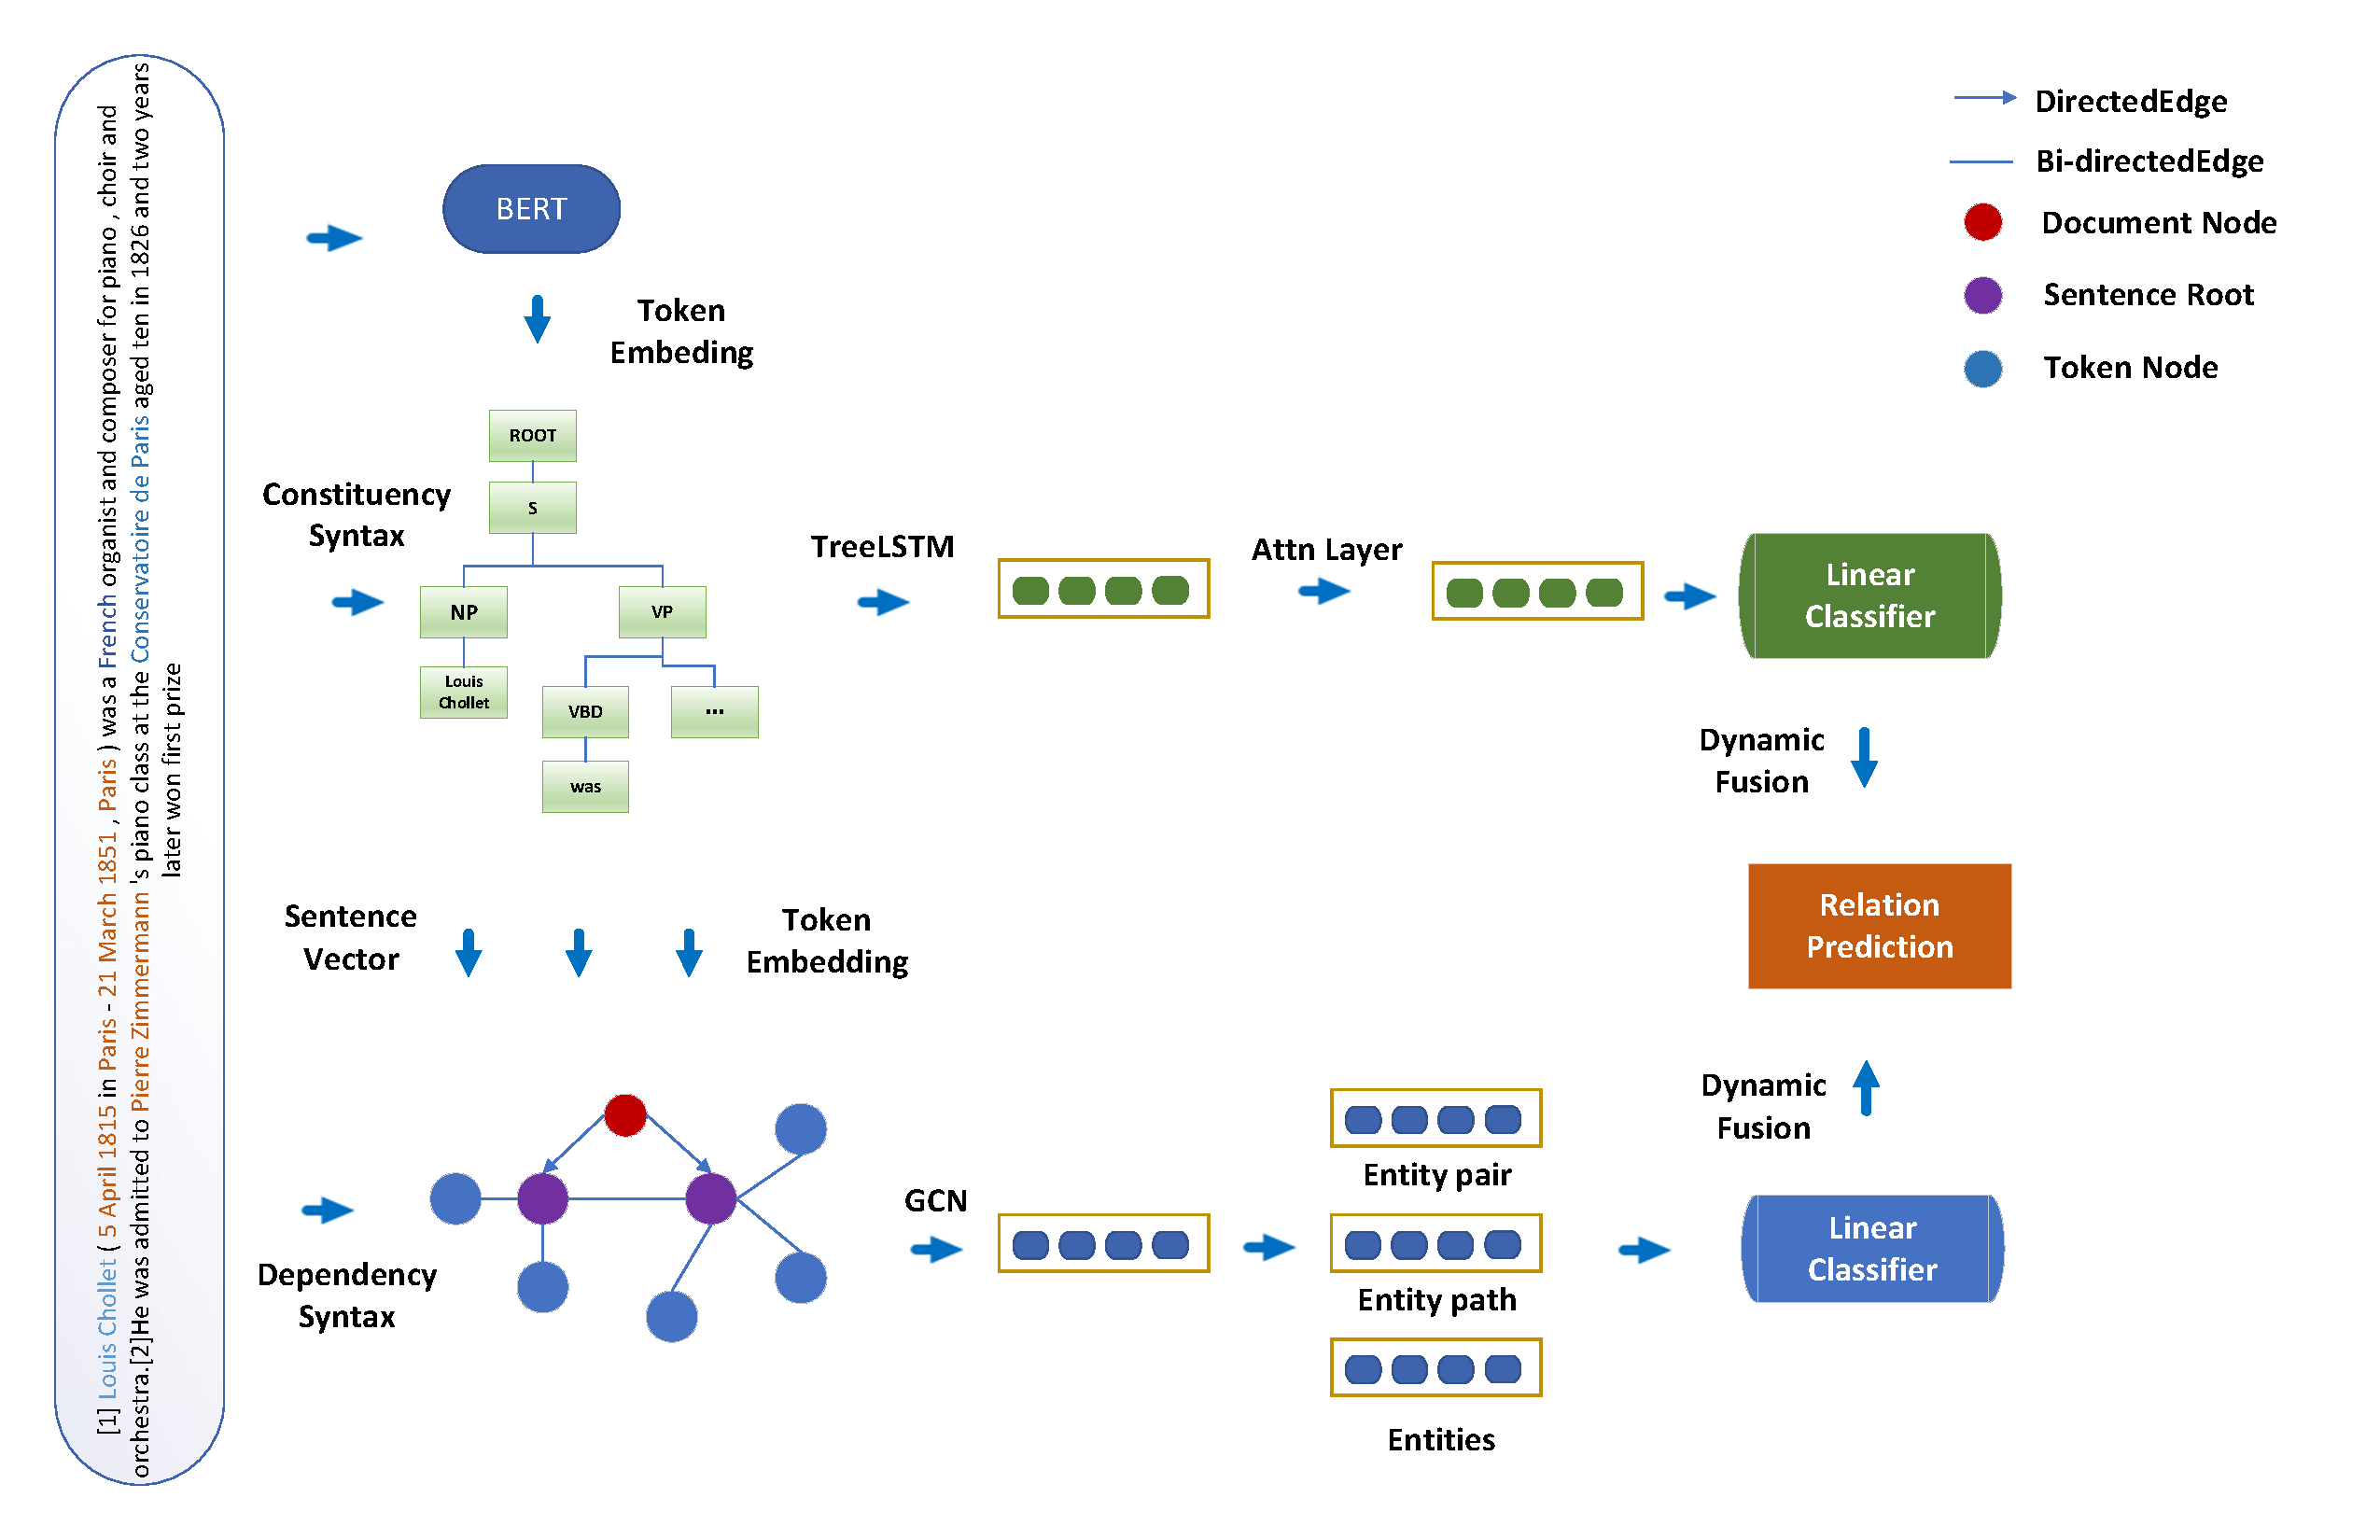
\includegraphics[height=0.5\linewidth]{misc/overview.pdf}}
    \caption{整体算法的概述。我们使用选区语法的结果来增强依赖图,并通过动态加权融合获得实体对之间的关系。}
\end{figure*}\label{overview}




    
\section{单词嵌入}

\section{基于依存语法树的文档级关系抽取}
\begin{figure}[t]
    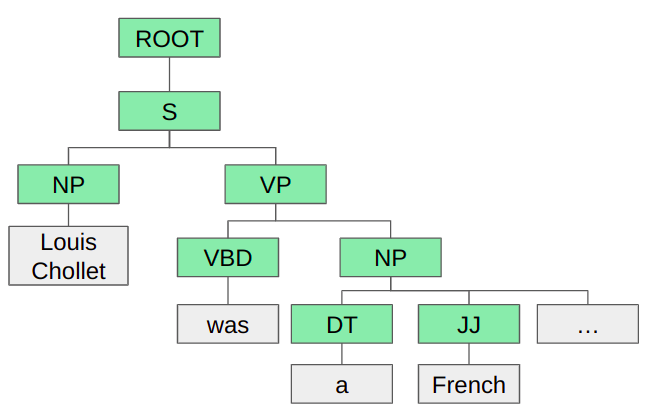
\includegraphics[width=0.5\textwidth]{misc/constituency.png}
    \caption{依存树将句子组织成树结构,不仅可以引入额外的层次语法信息,还可以在任意粒度上探索子内容。非叶节点颜色为绿色。} 
\end{figure}\label{fig_syn_b}

\section{基于依赖语法树的文档级关系抽取}
\begin{figure}[t]
    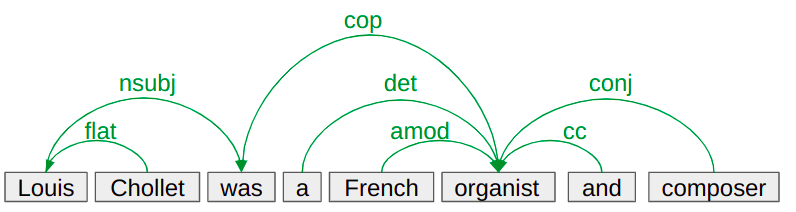
\includegraphics[width=0.5\textwidth]{misc/dependency.png}
    \caption{依赖语法树描述单个句子中单词之间的依赖关系。利用这样的语法信息可以显著地补充原始的纯文本,并捕捉相邻单词之间的关系。我们的模型将依赖树转换为依赖图。} 
\end{figure}\label{fig_syn_a}

\section{融合两种不同语法树结果的文档级关系抽取}
% 两页

\section{本章小结}
\newpage
1
\newpage


\chapter{基于语法树的文档级关系抽取实验结果}
为了全面的评估我们的模型,我们在来自不同领域的三个文档级数据集上评估了我们的算法模型。
我们在第 \ref{sec:dataset}节介绍了这些模型,在第 \ref{sec:docred}和 \ref{sec:medical}节说明了我们的结果。
然后,我们在第 \ref{sec:weight}节分析了两种不同的语法树权重,在第 \ref{sec:distance}节分析了依赖语法树路径距离。
最后,我们在第 \ref{sec:inter}节进行了消融实验,并总结了我们的研究结果。

\section{文档级关系抽取抽取数据集说明}\label{sec:dataset}

\begin{table}[h]
    \caption{三个公共数据集的统计数据}
    \begin{tabular}{cccc}
    \hline
    统计数据               & DocRED & CDR & GDA   \\ \hline
    \# 训练集                 & 3053   & 500 & 23353 \\
    \# 验证集                   & 1000   & 500 & 5839  \\
    \# 测试集                  & 1000   & 500 & 1000  \\
    \# 关系数量             & 96     & 2   & 2     \\
    \# 平均每篇文章的句子数量 & 8.0    & 9.7 & 10.2  \\ \hline
    \end{tabular}
\end{table} \label{table:datasets}
尽管文档级关系抽取方法可能因为要提取的关系类型(基因-疾病关系,一般类型的关系等)而有所不同,但大多数关系抽取方法都是在通用数据集和医学数据集上进行评估的。
因此我们选择了一个通用数据集和两个医学数据集来评估我们的模型,表 \ref{table:datasets}列出了这些数据集的统计数据。
\begin{itemize}
    \item \textbf{DocRED} \cite{DOCRED} 是一个从维基百科中人为标注的大型数据集。
    它包含从维基百科中采样的5053个黄金注释文档,132275个实体、56354个关系事实和96个关系类,每篇平均长度为196.7个单词,超过40.7\%的关系对是跨句关系事实。
    实体部分包括经典的实体标签,如PERSON、ORGANIZATION和LOCATION;而实体关系部分使用了96种关系类型,涵盖了广泛的科目, 包括科学(33.3\%)、艺术(11.5\%)、时间(8.3\%)、个人生活(4.2\%)等。
    \item \textbf{CDR} \cite{li2016biocreative} 是一个生物医学的文档级关系抽取数据集,由1500篇PubMed的摘要组成。
    这些摘要被随机分为三个相等的部分进行训练、验证和测试。
    这个数据集的预测任务是预测化学品和疾病之间的二元关系。
    \item \textbf{GDA} \cite{GDA} 
    也是一个生物医学的文档级关系抽取数据集,包含30192篇摘要。
    这个大型数据集是通过对公开数据库收集的基因-疾病关联中的30192篇摘要(测试集为1000篇,其余按80:20的比例在训练集和验证集之间划分)进行远程监督构建的。
    这个数据集的预测任务是预测基因和疾病之间的二元关系。
\end{itemize}

\section{DocRED数据集实验结果说明与分析}\label{sec:docred}

\section{医学数据集实验结果说明与分析}\label{sec:medical}

\section{两种不同的语法树权重分析}\label{sec:weight}

\section{依赖语法树路径距离分析}\label{sec:distance}

\section{消融实验结果说明与分析}\label{sec:inter}

\section{本章小结}\label{sec:conclusion}
\newpage
1
\newpage
\chapter{结论}
1
\begin{comment}
    在工作总结的基础上,经过分析、归纳,明确结论:
①系统功能、指标等是否实现或达到课题要求(工程技
术及软件课题)
②理论结果是否正确、所建模型是否合理(理论课题)
41③所阐述的观点是否正确(文科课题)
④本课题有待进一步解决的问题及方向
⑤本人收获及体会
\end{comment}
\thesisacknowledgement
在攻读计算机学士学位期间,首先热烈感谢我的导师康昭教授。经过风风雨雨的研究,我得到了他的无私关怀和支持。在此特别表达感谢之情。我还要感谢我的一直以来的帮助者们,包括学院的老师、同学、同事,以及所有支持和关心我的人。我也要感谢我的家人,他们给予我强大的内心支持和生活的安定和稳定。

% Uncomment to list all the entries of the database.
%\bibliography command
%\nocite{*}
%\thesisbibliography{reference}

%
% Uncomment following codes to load bibliography database with native
%\bibliography command.

\bibliographystyle{thesis-uestc}
\bibliography{reference}


%\thesistranslationoriginal
%\section{The OFDM Model of Multiple Carrier Waves}

%\thesistranslationchinese
%\section{基于多载波索引键控的正交频分多路复用系统模型}

\end{document}
